% !TEX program = lualatex
% !TEX spellcheck = it_IT
% !TEX root = ../campi.tex

\section{Gruppo di Galois}

\begin{defi}
Il {\em gruppo di Galois} di un'estensione \(i : K \to L\) è
\[\Gal{K \mor i L} := \{\sigma : L \to L \text{ automorfismo} \mid \sigma \circ i = i \} .\]
%\marginpar{
\begin{figure}
\centering
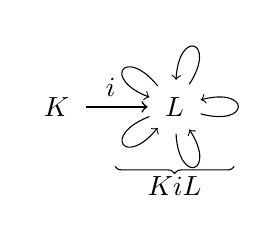
\begin{tikzpicture}
\pgfmathsetmacro\looprad{1}
\node [circle] (L) {\(L\)};
\node [rectangle, minimum size=1.5*\looprad cm] (Gal) at (L) {};
\foreach \i in {0, ..., 4} {
  \draw [->] (L) .. controls +(72*\i-15:\looprad) and +(72*\i+15:\looprad) .. (L);
}
\node [circle] (K) at +(180:{1.5*\looprad}) {\(K\)};
\draw [->, semithick] (K) to node[auto, pos=.4]{\(i\)} (L);
\draw [decoration={brace, mirror}, decorate] (Gal.south west) -- node[below]{\(\Gal{K \mor i L}\)} (Gal.south east);
\end{tikzpicture}
\caption{Il gruppo di Galois di un'estensione}
\end{figure}
%}
Qualche volta l'omomorfismo è chiaro dal contesto o è una semplice inclusione, quindi non ci si scomoda a dargli un nome: alcune notazioni alternative sono \(\Gal{K \hookrightarrow L}\), \(\Gal{K \subseteq L}\), \(\Gal{L/K}\) oppure \(\Gal[K]{L}\).
\end{defi}

Cioè il gruppo di Galois di \(i : K \to L\) è il gruppo degli automorfismi \(L \to L\) che fissano gli elementi dell'immagine di \(K\) in \(L\). Se usiamo il solito abuso, possiamo dire che è il gruppo degli automorfismi di \(L\) che fissano gli elementi di \(K\), il che non scatena grossi intoppi in molti casi concreti.

In generale, il gruppo di Galois può essere complicato da calcolare: partiamo quindi dai casi in cui per lo meno abbiamo qualche appiglio a cui appoggiarsi, come il gruppo di Galois di un'estensione semplice e finita.

\begin{prop}\label{prop:GalEstensioneSempliceFinita}
Sia \(i : K \to L = K(\alpha)\) un'estensione semplice e \(m \in K[X]\) polinomio minimo di \(\alpha\). Allora esiste una corrispondenza biunivoca tra l'insieme delle radici di \(m\) in \(L\) e l'insieme degli elementi di \(\Gal[K]L\): la funzione
\[\{\text{radici di \(m\) in \(L\)}\} \to \Gal[K]L \]
che manda una radice \(\gamma\) in \(L\) nell'automorfismo che manda \(\alpha\) in \(\gamma\). In particolare \(\Gal[K]L\) ha cardinalità \(\le [L:K] = \deg m\) e vale l'uguaglianza se e solo se \(m\) ha \(\deg m\) radici distinte in \(L\).
\end{prop}

\begin{proof}
Tutto il lavoro è fatto nel Corollario~\ref{coro:NumeroMorfismiEstensioniDaKAlgebrico}. \nota{Quasi: scrivere anche come mai gli endomorfismi di estensioni finite sono automorfismi.}
\end{proof}

La Proposizione dice precisamente quali sono gli elementi del gruppo e la sua cardinalità in un certo caso. È importante notare tuttavia che gruppi con la stessa cardinalità non necessariamente sono isomorfi, quindi la Proposizione sopra da qualche indicazione ma in generale non risolve totalmente il problema della determinazione del gruppo di Galois: dei conti vanno fatti e della Teoria dei Gruppi Finiti può sempre far comodo.

Un caso fortunato è quello in cui il gruppo di Galois ha ordine primo: in questo caso, il gruppo di Galois è ciclico è la questione è immediatamente dipanata.

\begin{esem}[Gruppo di Galois di \(\Q \subseteq \Q(i)\)]
Il numero complesso \(i\) ha polinomio minimo \(X^2+1 \in \Q[X]\). Notiamo anche che \(\Q(i)\) contiene entrambe le radici, \(i\) e \(-i\), e che queste sono tutte distinte. Quindi \(\card{\Gal{\Q \subseteq \Q(i)}} = 2\). Il gruppo di Galois è quindi (isomorfo a) \(C_2\). Scriviamo comunque gli automorfismi esplicitamente: uno è quello che manda \(i\) in \(i\) ed è l'identità, mentre l'altro manda \(i\) in \(-i\). Ricordando che si può scrivere \(\Q(i) = \{a+bi \mid a, b \in \Q\}\), si ha che quest'ultimo automorfismo è
\[\Q(i) \to \Q(i)\,,\ a+bi \mapsto a-bi .\]
\end{esem}

%\begin{esem}[Gruppo di Galois di \(\Q \subseteq \Q(i)\)]
%Prendiamo un generico \(\phi \in \Gal{\Q \subseteq \Q(i)}\) e cerchiamo di capire cosa fa. Da definizione, gli elementi di \(\Q\) vengono tenuti fissi.
%%Per la Proposizione sopra, rimane da capire dove viene mandato \(i\). 
%Ricordiamo che \(i\) ha polinomio minimo \(X^2+1 \in \Q[X]\) e quindi \(\Q(i) = \{ a+bi \mid a, b \in \Q \}\) per il Corollario~\ref{coro:KAlgebricoEsplicito}. Quindi
%\[\phi (a+bi) = a+b\phi(i) .\]
%Rimane quindi da capire dove viene mandato \(i\). Poiché \(i^2 = -1\), si ha
%\[-1 = \phi(-1) = \phi\left(i^2\right) = \phi(i)^2\]
%da cui \(\phi(i) = \pm i\).
%%con l'obbiettivo di determinare \(a, b \in \Q\) opportuni. Sicuramente \(b \ne 0\), perché se fosse \(b = 0\) avremmo che \(\phi(i) = a \in \Q\), ma questo non può essere. Calcoliamo \(\phi\left(i^2\right)\) per esempio:
%%\[\phi\left(i^2\right) = \phi(i)^2 = a^2 - b^2 + 2abi .\]
%%Qui \(\phi\left(i^2\right) = \phi(-1) = -1\) perché \(\phi\) è un automorfismo che fissa gli elementi di \(\Q\). Quindi
%%\[-1 = a^2 - b^2 + 2abi .\]
%%Osserviamo che deve essere \(a = 0\): perché in caso contrario si avrebbe
%%\[\underbrace{\frac{-1-a^2+b^2}{2ab}}_{\in \Q} = \underbrace{i}_{\notin \Q} .\]
%%Quindi \(\phi(i) = bi\).  Elevando al quadrato, come abbiamo già fatto, si ha che \(-1 = -b^2\), cioè \(b = \pm 1\). 
%Quindi l'automorfismo \(\phi\) è quello che manda \(i\) in \(i\)
%\[\phi(a+bi) = a+bi\]
%oppure quello che manda \(i\) in \(-i\)
%\[\phi(a+bi) = a-bi .\]
%Il gruppo di Galois dell'estensione \(\Q \subseteq \Q(i)\) è isomorfo a \(\Z/2\Z\). 
%\end{esem}

\begin{eser}
Studiare il gruppo di Galois di \(\Q \subseteq \Q\left(\sqrt2\right)\).
\end{eser}

Vediamo qualche esempio in cui bisogna operare delle scelte. Ricordiamo a tal proposito che se \(G\) è un gruppo di ordine \(p^2\) con \(p\) primo, allora \(G\) è isomorfo a \(C_{p^2}\) oppure a \(C_p \times C_p\).

\begin{esem}
Calcoliamo il gruppo di Galois dell'estensione \(\Q \subseteq L := \Q\left(\sqrt 2, \sqrt 3\right)\). Come abbiamo visto, \(L = \Q(\alpha)\), con \(\alpha := \sqrt2+\sqrt3\), e il polinomio minimo di \(\alpha\) è \(f := X^4-10X^2+1 \in \Q[X]\). Questo polinomio ha 4 radici distinte tutte in \(L\), che sono:
\[-\sqrt3-\sqrt2 \,,\ -\sqrt3+\sqrt2 \,,\ \sqrt3-\sqrt2 \,,\ \sqrt3+\sqrt2 .\]
Quindi il gruppo di Galois ha cardinalità \(4\), per cui le possibilità sono due: e isomorfo a \(C_4\) oppure a \(C_2 \times C_2\). Quale delle due? La proposizione sopra ci dice chi sono gli elementi del gruppo di Galois, che sono determinati da quale radice di \(f\) è mandato \(\sqrt2+\sqrt3\). Ecco il piano: se il gruppo di Galois contiene qualche elemento di ordine \(4\), allora è \(C_4\), altrimenti è \(C_2 \times C_2\).\newline
L'automorfismo \(\sigma_1\) che manda \(\alpha\) in \(\alpha\) è l'identità, quindi la mettiamo da parte. Vediamo l'automorfismo \(\sigma_2\) che manda \(\alpha\) in \(-\sqrt3-\sqrt2\).
\[\alpha \mor{\sigma_2} -\alpha \mor{\sigma_2} - \sigma_2 (\alpha) = \alpha\]
e quindi l'ordine di \(\sigma_2\) è \(2\). Vediamo l'automorfismo \(\sigma_3\) che manda \(\alpha\) in \(-\sqrt3+\sqrt2 = -\frac{1}{\alpha}\).
\[\alpha \mor{\sigma_3} -\frac{1}{\alpha} \mor{\sigma_3} - \frac{1}{\sigma_3 (\alpha)} = \alpha\]
e quindi l'ordine di \(\sigma_3\) è ancora \(2\). Vediamo l'automorfismo \(\sigma_4\) che manda \(\alpha\) in \(\sqrt3-\sqrt2 = \frac{1}{\alpha}\).
\[\alpha \mor{\sigma_4} \frac{1}{\alpha} \mor{\sigma_4} \frac{1}{\sigma_4 (\alpha)} = \alpha\]
e quindi l'ordine di \(\sigma_3\) è ancora \(2\). Possiamo concludere che \(\Gal[\Q]L \iso C_2 \times C_2\).
%Facciamo una tabella per elencarli tutti.
%Facciamo una tabella per elencarli tutti.
%\[\begin{array}{c|c|c|c|c}
%         &  -\sqrt3-\sqrt2 & -\sqrt3+\sqrt2 & \sqrt3-\sqrt2 & \sqrt3+\sqrt2 \\
%\sigma_1 & & & & -\sqrt3-\sqrt2 \\
%\sigma_2 & & & & -\sqrt3+\sqrt2 \\
%\sigma_3 & & & & \sqrt3-\sqrt2  \\
%\sigma_4 & & & & \sqrt3+\sqrt2
%\end{array}\]
\end{esem}

Non siamo così fortunati in generale per le estensioni finitamente generate, anche se abbiamo una proprietà che restringe il campo di ricerca degli elementi dei gruppi di Galois.

\begin{prop}
Sia \(i : K \to L\) un'estensione finitamente generata, cioè \(L = K\left(\alpha_1, \dots{}, \alpha_n\right)\) per degli \(\alpha_1, \dots{}, \alpha_n \in L\). Ogni \(\phi \in \Gal[K]{L}\) è univocamente determinato da \(\phi\left(\alpha_1\right), \dots{}, \phi\left(\alpha_n\right)\). In particolare, \(\Gal[K]{L}\) è isomorfo ad un sottogruppo di \(S_n\).
\end{prop}

\begin{proof}
Da definizione, gli elementi di \(\Gal[K]{L}\) fissano gli elementi di \(K\) e se due elementi di \(\Gal[K]{L}\) sono uguali su \(\left\{\alpha_1, \dots{}, \alpha_n\right\}\), allora sono uguali ovunque.
\end{proof}

%\begin{coro}
%Sia \(i : K \to L\) un'estensione finitamente generata, cioè \(L = K\left(\alpha_1, \dots{}, \alpha_n\right)\) per degli \(\alpha_1, \dots{}, \alpha_n \in L\). Allora \(\Gal[K]{L}\) è isomorfo ad un sottogruppo di \(S_n\).
%\end{coro}

E qui è chiaro anche come mai ci sia un interesse verso i gruppi simmetrici \(S_n\) e i suoi sottogruppi, perché sostanzialmente gli elementi di \(\Gal[K]{L}\) sono permutazioni degli \(\alpha_i\).

\begin{prop}
Sia \(i : K \to L\) un'estensione, \(f \in K[X]\) e \(\phi \in \Gal[K]{L}\). Allora per ogni \(\alpha \in L\) si ha
\[i_\ast(f)(\phi(\alpha)) = \phi\left(i_\ast(f)(\alpha)\right) .\]
Quindi gli elementi di \(\Gal[K]L\) mandano le radici di \(f\) in \(L\) in radici di \(f\) in \(L\). %e \(\Gal[K] f\) è isomorfo ad un sottogruppo delle permutazioni delle radici di \(f\).
\end{prop}

\begin{proof}
Scriviamo \(f := \sum_{k \in \N} a_k X^k\) e ricordiamo che \(\phi \circ i = i\).
\begin{align*}
i_\ast (f) (\phi(\alpha)) &= \sum_{k \in \N} i\left(a_k\right) (\phi(\alpha))^k = \\
                          &= \sum_{k \in \N} \phi\left(i\left(a_k\right)\right) \phi\left(\alpha^k\right) = \\
                          &= \phi\left( \sum_{k \in \N} i\left(a_k\right) \alpha^k \right) = \\
                          &= \phi\left(i_\ast(f)(\alpha)\right) .\qedhere
\end{align*}
\end{proof}

Perché questo è importante? Per questo motivo ad esempio.

\begin{coro}
Sia \(i : K \to L = K\left(\alpha_1, \dots{}, \alpha_n\right)\) un'estensione finitamente generata e \(m_1, \dots{}, m_n \in K[X]\) polinomio di minimi di \(\alpha_1, \dots{}, \alpha_n\) rispettivamente. Allora gli elementi di \(\Gal[K]L\) per ogni \(i \in \{1, \dots, n\}\) mandano \(\alpha_i\) in radici di \(m_i\) in \(L\).
\end{coro}

%\begin{prop}
%\(F\subseteq K\subseteq L\) estensioni con \(F\subseteq L\) finita e normale. \\
%Allora \(F\subseteq K\) è normale \(\iff\) \(K\) è \(\Gal[F]{L}\)-stabile (cioè \(\sigma(K)=K\) \(\all\sigma\in\Gal[F]{L}\), o, equivalentemente, \(\sigma(K)\subseteq K\) \(\all\sigma\in\Gal[F]{L}\)).
%\end{prop}
%
%\begin{proof}
%\begin{itemize}
%\item[\(\implies\)] \(\sigma\in\Gal[F]{L}\) \(\implies\) \(\sigma(K)\subseteq K\):
%\smallskip
% 
%\(\alpha\in K\) \(\implies\) \(\polmin_{\alpha,F}(\sigma(\alpha))=\sigma(\polmin_{\alpha,F}(\alpha))=\sigma(0)=0\) \(\implies\) \(\sigma(\alpha)\in K\) perché \(\polmin_{\alpha,F}\) si spezza su \(K\).
%\item[\(\impliedby\)] \(F\subseteq L\) normale e finita \(\implies\) \(F\subseteq L\) campo di spezzamento di \(f\in F[X]\setminus\{0\}\).
%\smallskip
%
%\(\alpha\in K\) \(\implies\) \(\polmin_{\alpha,F}\) si spezza su \(L\), e va dimostrato che si spezza su \(K\), cioè che \(\beta\in L\) tale che \(\polmin_{\alpha,F}(\beta)=0\) \(\implies\) \(\beta\in K\).
%\smallskip
%
%\(\exiun\) \(F\)-omomorfismo \(i : F(\alpha)\to L\) tale che \(i(\alpha)=\beta\). \\
%\(F(\alpha)\subseteq L\) campo di spezzamento di \(f\), \(f=i(f)\) si spezza su \(L\) \(\implies\) \(\exi\) \(F(\alpha)\)-omomorfismo (e quindi \(F\)-omomorfismo) \(\sigma : L\to L\) (cioè tale che \(\sigma\rest{F(\alpha)}=i\)).
%\smallskip
%
%\(\sigma(L)\subseteq L\), \(\dim_F(\sigma(L))=\dim_F(L)<\infty\) \(\implies\) \(\sigma(L)=L\) \(\implies\) \(\sigma\in\Gal[F]{L}\) \(\implies\) \(\beta=i(\alpha)=\sigma(\alpha)\in\sigma(K)=K\).\qedhere
%\end{itemize}
%\end{proof}

\begin{defi}
Sia \(K\) un campo, e \(f \in K[X]\) non nullo. Il {\em gruppo di Galois} di \(f\) su \(K\) è il gruppo di Galois di un campo di spezzamento per \(f\). Viene indicato molto semplicemente come \(\Gal[K] f\).
%(ben definito a meno di isomorfismo) è \(\Gal[K]{f}:=\Gal[K]{L}\) con \(K\subseteq L\) campo di spezzamento di \(f\).
\end{defi}

Abbiamo visto che il campo di spezzamento è unico a meno di isomorfismo, e anche il corrispondente gruppo di Galois è definito a meno di isomorfismo. È importante capire che è importante avere una certa manualità nel calcolo dei campi di spezzamento di polinomi.

\begin{coro}
Sia \(K\) un campo e \(f \in K[X]\) non nullo. Allora \(\Gal[K] f\) è isomorfo ad un sottogruppo delle permutazioni delle radici di \(f\) e in particolare, se \(f\) ha \(d\) radici distinte, allora \(\card{\Gal[K]f}\) divide \(d!\).
\end{coro}

%\begin{coro}
%Sia \(K\) un campo e \(f \in K[X]\) non nullo con \(d\) radici distinte in qualche suo campo di spezzamento. Allora \(\card{\Gal[K]f}\) divide \(d!\).
%\end{coro}

Per polinomi di grado piccolo, \(2\) oppure \(3\), questo è interessante.

\begin{esem}[Gruppo di Galois di polinomi di secondo grado]
\nota{Nessun problema per quanto riguarda la caratteristica di \(K\)?} Sia \(K\) un campo e \(f := aX^2+bX+c \in K[X]\). Se \(f\) ha una sola radice distinta, allora \(\Gal[K]f\) deve essere necessariamente banale. Se invece, ha due radici distinte, allora le possibilità sono due: \(\Gal[K]f\) è banale oppure ha ordine \(2\), cioè è ciclico di ordine \(2\). Vediamo quando accade ciò.
%Ricordiamo prima che se \(f = a(X-\alpha_1)(X-\alpha_2)\), allora \(\alpha_1\) e \(\alpha_2\) sono entrambe in \(K\) oppure entrambe non in \(K\). I casi sono quindi due:
\begin{itemize}
\item \(f\) è riducibile su \(K[X]\), e quindi ha due radici \(K\). In questo caso il campo di spezzamento è \(K\) stesso e il gruppo di Galois di \(f\) è banale.
\item \(f\) è irriducibile su \(K[X]\), e quindi non ha radici \(K\). Dobbiamo ricorrere ad un campo di spezzamento \(K \subseteq K(\alpha_1, \alpha_2)\) che per il Teorema~\ref{teor:EsistenzaCampoSpezzamento} ha grado \(2\). Pure il sottospazio \(K(\alpha_1)\) ha grado \(2\) perché il polinomio minimo di \(\alpha_1\) ha grado \(2\). Quindi \(K(\alpha_1, \alpha_2) = K(\alpha_1) = \{a+b\alpha_1 \mid a, b \in K\}\). Il gruppo di Galois allora contiene, oltre all'identità, sicuramente l'automorfismo che manda \(\alpha_1\) in \(\alpha_2\). Il gruppo di Galois quindi è (a meno di isomorfismi) \(C_2\).
\end{itemize}
%Richiamiamo come si possono calcolare le radici di \(f\):
%\[\frac{-b + \sqrt{b^2-4ac}}{2a} \quad \frac{-b + \sqrt{b^2-4ac}}{2a} .\]
%Quindi, se ha radici distinte, allora sono entrambe reali oppure con parte immaginaria non nulla. Nel primo caso, il campo di spezzamento è \(Q\)
\end{esem}

\begin{eser}
Al variare di \(K\) potrebbe variare anche il gruppo di Galois. Calcolare, ad esempio, \(\Gal[\Q]{X^2-2}\) e \(\Gal[\R]{X^2-2}\).
\end{eser}

\begin{esem}[Gruppo di Galois di polinomi di terzo grado]
\nota{\dots}
\end{esem}

Fortunatamente riusciamo ancora ad avere ancora qualche indicazione sulla cardinalità del gruppo di Galois per estensioni finite.

\begin{lemm}\label{lemm:NumeroMorfismiEstensioniDaEstensioneFinita}
Sia \(i : K \to L\) un'estensione finita e \(j : K \to L'\) un'altra estensione. Allora il numero dei morfismi di estensioni \(L \to L'\) da \(i\) a \(j\) è \(\le [L:K]\). Inoltre vale l'uguaglianza se e solo se per ogni \(\alpha \in L\) il suo polinomio minimo come elemento di \(L'[X]\) si spezza ed è separabile.
%\(\polmin_{\alpha,K}\) ha \(\deg(\polmin_{\alpha,K})\) radici distinte in \(L'\) (cioè \(\polmin_{\alpha,K}\) è separabile e si spezza su \(L'\)) \(\all\alpha\in L\).
\end{lemm}

\begin{proof}
A causa della Proposizione~\ref{prop:EstensioneFinitaEquivalenti}, se \(i : K \to L\) è finita, allora esistono \(\alpha_1, \dots{}, \alpha_n \in L\) algebrici tali che \(L = K\left(\alpha_1, \dots{}, \alpha_n\right)\). Andiamo a dimostrare per induzione sul numero \(n\) di generatori \(\alpha_i \in L\) il seguente fatto:
\begin{quotation}
Sia \(i : K \to L = K\left(\alpha_1, \dots{}, \alpha_n\right)\) un'estensione con \(\alpha_1, \dots{}, \alpha_n\) algebrici e \(j : K \to L'\) un'altra estensione. Allora il numero dei morfismi di estensioni \(L \to L'\) da \(i\) a \(j\) è \(\le [L:K]\). Vale l'uguaglianza se e solo se ogni \(\alpha_i \in L\) ha un polinomio minimo si spezza in \(L'[X]\) ed è separabile.
\end{quotation}
Il caso base, \(n=1\), è La Proposizione~\ref{prop:GalEstensioneSempliceFinita}. Sia ora \(n > 0\). Introduciamo il campo \(E := K\left(\alpha_1, \dots{}, \alpha_{n-1}\right)\), per cui \(L = E(\alpha_n)\), e decomponiamo l'estensione \(i : K \to L\) come segue
\[\begin{tikzcd}[column sep=small]
K \ar["i", rr] \ar["{i_1}", dr, swap] & & L \\
& E \ar["{i_2}", ur, swap]
\end{tikzcd}\]
dove \(i_1(r) := i(r)\) e \(i_2(s) := s\). Disegniamo allora
\[\begin{tikzcd}
E\left(\alpha_n\right) & & L' \\
E \ar["{i_2}", u] \\
& K \ar["{i_1}", ul] \ar["j", uur, swap]
\end{tikzcd}\]
Induttivamente, ci sono al massimo \([E:K]\) morfismi di estensioni da \(i_1\) a \(j\) e per ciascuno dei siffatti \(h : E \to L'\), grazie al Corollario~\ref{coro:NumeroMorfismiEstensioniDaKAlgebrico}, sappiamo che il numero di morfismi di estensioni da \(i_2\) a \(h\)
\[\begin{tikzcd}
E(\alpha_n) \ar[r] & L' \\
E \ar["{i_2}", u] \ar["h", ur, swap]
\end{tikzcd}\]
è minore o uguale a \(\left[E\left(\alpha_n\right):E\right]\). Per costruzione questi morfismi di estensioni sono morfismi da \(i\) a \(j\). Quindi al massimo ci sono
\[[E(\alpha_n):E][E:K] = [L:E][E:K] = [L:K]\]
estensioni da \(i\) a \(j\). È immediato anche constatare come se i polinomi minimi si spezzano su \(L'\) e sono separabili, allora il numero dei morfismi di estensioni è esattamente \([L:K]\). Per il viceversa, supponiamo che ci siano \([L:K]\) morfismi di estensioni da \(i\) a \(j\). \nota{Qui è da riscrivere meglio\dots{}}
\end{proof}

\begin{defi}
Un'estensione è detta {\em di Galois} qualora è finita, normale e separabile. Equivalentemente, un'estensione è di Galois quando è campo di spezzamento di un qualche polinomio non nullo separabile.
\end{defi}

Il Lemma sopra fornisce quindi un criterio che può essere comodo a volte per capire se un'estensione \(K \subseteq L\) è di Galois, a patto di avere l'informazione della cardinalità di \(\Gal[K]{L}\).

\begin{prop}[Cardinalità gruppi di Galois]\label{prop:CardGruppiGalois}
Se \(K \subseteq L\) è un'estensione finita, allora \(\card{\Gal[K]{L}} \le [L:K]\). Vale l'uguaglianza se e solo se l'estensione è di Galois.
\end{prop}

\begin{proof}
Poiché \(K \subseteq L\) è un'estensione finita, allora i morfismi di estensioni da \(K \subseteq L\) sono tutti automorfismi. Ricordiamo infatti che i morfismi di estensioni sono applicazioni lineari se si vede \(L\) come spazio vettoriale su \(K\) di dimensione finita. Allora \(\Gal[K]{L}\) è il gruppo dei morfismi di estensione dall'estensione \(K \subseteq L\) in sé: si applica il Lemma di sopra.
\end{proof}

Quindi il gruppo di Galois di un'estensione finita è finito: l'interesse per i gruppi di ordine finito risiede anche in questo. \nota{Fare qualche esempio in cui il gruppo di Galois è infinito.}

\begin{prop}
Se \(F \subseteq K \subseteq L\) sono estensioni con \(F \subseteq L\) di Galois, allora anche \(K\subseteq L\) è di Galois.
\end{prop}

\begin{proof}
\nota{Ancora da scrivere.}
\end{proof}

%\begin{osse}
%\(K\subseteq L\) campo di spezzamento di \(f\in K[X]\setminus\{0\}\), \(G:=\Gal[K]{f}\).
%\begin{itemize}
%\item \(K\) perfetto \nota{parlare dei campi perfetti} \(\implies\) \(K\subseteq L\) di Galois \(\implies\) \(\card{G}=[L:K]\).
%\item \(R:=\{\alpha\in L\st f(\alpha)=0\}\) \(\implies\) \(n:=\card{R}\le\deg(f)\). \\
%\(\sigma\in G\), \(\alpha\in R\) \(\implies\) \(\sigma(\alpha)\in R\), quindi si ottiene una funzione \(G\to S(R)\iso S_n\), \(\sigma\mapsto\sigma\rest{R}\), che è un omomorfismo iniettivo (perché \(L=K(R)\)) \(\implies\) \(G\iso G'< S_n\) (\(\implies\) \(\card{G}\dvd n!\)).
%\item \(K\) perfetto, \(f\) irriducibile \(\implies\) \(\deg(f)=n\) e \(n\dvd\card{G}\dvd n!\).
%\end{itemize}
%\end{osse}

\begin{osse}
Un caso particolarmente fortunato è quello dei campi perfetti. Abbiamo visto infatti che se \(K\) è perfetto, allora le estensioni algebriche \(K \subseteq L\) sono tutte separabili. Se con \(K \subseteq L\) è il campo di spezzamento di un certo \(f \in K[X]\) non nullo, allora \(K \subseteq L\) è di Galois. Se scriviamo \(G\) il gruppo di Galois di questa estensione, e \(\card G = [L:K]\) e \(\card G\) divide \((\deg f)!\); se inoltre \(f\) è pure irriducibile, possiamo dire anche che \(\deg f\) divide \(\card G\).
\end{osse}

%\begin{esem}
%Esempi: \(K\) perfetto, \(f\in K[X]\) irriducibile, \(n:=\deg(f)\), \(G:=\Gal[K]{f}\).
%\begin{itemize}
%\item \(n=2\) \(\implies\) \(2\dvd\card{G}\dvd2!\) \(\implies\) \(\card{G}=2\) \(\implies\) \(G\iso C_2\).
%\item \(n=3\) \(\implies\) \(3\dvd\card{G}\dvd3!\) \(\implies\) \(\card{G}=3\) o \(6\) \(\implies\) \(G\iso C_3\) o \(S_3\) (perché \(G\iso G'<S_3\)).\newline
%\(f=X^3-2\) \(\implies\) \(G\iso S_3\) se \(K=\Q\), \(G\iso C_3\) se \(K=\Q(\omega)\).
%\item \(n=4\) \(\implies\) \(4\dvd\card{G}\dvd4!\) \(\implies\) \(\card{G}=4\), \(8\), \(12\) o \(24\) \(\implies\) \(G\iso C_4\), \(C_2^2\), \(D_4\), \(A_4\) o \(S_4\) (perché \(G\iso G'<S_4\)).\newline
%\(f=X^4-10X^2+1=\polmin_{\alpha,\Q}\) con \(\alpha=\sqrt{2}+\sqrt{3}\) \(\implies\) \(G\iso C_2^2\): \(\Q\subset\Q(\alpha)=\Q(\sqrt{2},\sqrt{3})\) normale (perché campo di spezzamento di \((X^2-2)(X^2-3)\)) \(\implies\) \(f\) si spezza su \(\Q(\alpha)\) \(\implies\) \(\Q\subset\Q(\alpha)\) campo di spezzamento di \(f\) \(\implies\) \(G=\Gal[\Q]{\Q(\alpha)}\) \(\implies\) \(\card{G}=[\Q(\alpha):\Q]=\deg{f}=4\) e \(G\niso C_4\) perché \(\sigma\in G=\Gal[\Q]{\Q(\sqrt{2},\sqrt{3})}\) \(\implies\) \(\sigma(\sqrt{2})=\pm\sqrt{2}\) e \(\sigma(\sqrt{3})=\pm\sqrt{3}\) \(\implies\) \(\sigma^2(\sqrt{2})=\sqrt{2}\) e \(\sigma^2(\sqrt{3})=\sqrt{3}\) \(\implies\) \(\sigma^2=\id_{\Q(\sqrt{2},\sqrt{3})}\).
%\end{itemize}
%\end{esem}

\begin{eser}
Determinare il campo di spezzamento e il gruppo di Galois di \(f := X^4-4X^2+2\) su \(\Q\).
\end{eser}

\begin{proof}[Svolgimento]
Anzitutto \(f\) è irriducibile per il Criterio di Eisenstein. In particolare, è anche monico, quindi è il polinomio minimo delle sue radici in qualche campo di spezzamento (vedi Proposizione~\ref{prop:EquivalentiPolinomioMinimo}). Le radici di \(f\) sono \(\pm\alpha,\pm\beta\) con \(\alpha := \sqrt{2+\sqrt{2}}\) e \(\beta := \sqrt{2-\sqrt{2}}\) e possiamo scrivere il campo di spezzamento \(\Q \subseteq L := \Q(\alpha,\beta)\). Tuttavia osserviamo che è sufficiente un solo generatore, perché
\[\beta = \sqrt{2-\sqrt2} \frac{\sqrt{2+\sqrt2}}{\sqrt{2+\sqrt2}} = \frac{\sqrt2}{\alpha} = \underbrace{\frac{\alpha^2-2}{\alpha}}_{\in \Q(\alpha)} .\]
Quindi \(L = \Q(\alpha)\). Scriviamo \(G\) il gruppo di Galois dell'estensione in esame. Dato che \(\Q \subseteq L\) è di Galois (\(\Q\) perfetto e \(\Q \subseteq L\) campo di spezzamento) possiamo dirne la cardinalità
\[\card G = [L:\Q] = \deg f = 4 .\]
Grazie al Corollario~\ref{coro:NumeroMorfismiEstensioniDaKAlgebrico}, sappiamo che c'è un \(\sigma \in G\) tale che \(\sigma(\alpha) = \beta\). Riusiamo la relazione che abbiamo ricavato sopra tra \(\alpha\) e \(\beta\):
\[
\sigma^2(\alpha)=\sigma(\beta)=\sigma\left(\frac{\alpha^2-2}{\alpha}\right)=\frac{\beta^2-2}{\beta}=\frac{-\sqrt{2}}{\beta}=-\alpha
\]
Quindi \(\sigma^2 \ne \id_L\). Questo è importante perché \(\card G = 4\): quindi \(\sigma\) ha ordine \(4\). Possiamo concludere che \(G \iso C_4\).
\end{proof}

\begin{eser}
Determinare il campo di spezzamento e il gruppo di Galois di \(f := X^4-4X^2-2\) su \(\Q\).
\end{eser}

\begin{proof}[Svolgimento]
Per il Criterio di Eisenstein \(f\) è irriducibile. Inoltre è monico, quindi è il polinomio minimo delle sue radici in qualche campo di spezzamento. Le radici di \(f\) sono 
\[\pm \sqrt{2 \pm \sqrt6} .\]
Per semplicità, \(\alpha := \sqrt{\sqrt{6}+2}\) e \(\beta := \sqrt{\sqrt{6}-2}\). Quindi il campo di spezzamento è \(L = \Q(\alpha,\beta i)\). Vediamo di trovare dei generatori più comodi o addirittura di ridurli. Osserviamo che \(\alpha \beta i = \sqrt2 i\) e quindi \(\sqrt2 i \in L\). Possiamo scrivere che \(L = \Q\left(\alpha, \sqrt2 i\right)\). L'estensione \(\Q \subseteq L\) è di Galois la stessa ragione dell'esercizio precedente. Calcoliamo il grado dell'estensione \(\Q \subseteq L\).
\[[L:\Q] = \left[\Q\left(\alpha, \sqrt2i\right):\Q(\alpha)\right] [\Q(\alpha):\Q] .\]
Qui, \([\Q(\alpha):\Q]\) è facile da calcolare, fa \(\deg f = 4\). Rimane il grado dell'altra estensione, che è \(2\) (esercizio per te!). Quindi \(\card G = 8\). Siamo fortunati perché questo ci basta: \(G\) si può identificare con un sottogruppo di \(S_4\) e l'unico sottogruppo di \(S_4\) che ha ordine \(8\) è il {\em gruppo diedrale} di ordine \(8\)
\[D_4 := \gen{r, s \left\mid r^4 = s^2 = (sr)^2 = 1\right.} .\qedhere\]
%\(\alpha\beta=\sqrt{2}\) \(\implies\) \(\alpha\beta i=\sqrt{2}i\) \(\implies\) \(L=\Q(\alpha,\sqrt{2}i)\). \\
%\([\Q(\alpha):\Q]=\deg(\polmin_{\alpha,\Q})=\deg(f)=4\), \([\Q(\sqrt{2}i):\Q]=\deg(\polmin_{\sqrt{2}i,\Q})=2\) (perché \(\polmin_{\sqrt{2}i,\Q}=X^2+2\)) \(\implies\) 
%\[
%\mcm(4,2)=4\dvd\card{G}=[\Q(\alpha,\sqrt{2}i):\Q]\le4\cdot2=8
%\]
%e non pu\`o essere \([\Q(\alpha,\sqrt{2}i):\Q]=4\) (perché \(\sqrt{2}i\not\in\Q(\alpha)\subset\R\)) \(\implies\) \(\card{G}=8\). \\
%\(G\iso G'<S_4\) \(\implies\) \(G\iso D_4\).
\end{proof}

\begin{osse}
Come vedi, qualche nozione sui gruppi finiti serve sempre.
\end{osse}

\begin{eser}[Problema 231 di~\cite{tsumura:exercises}]
Far vedere che \(\Q \subseteq \Q\left(\sqrt{2+\sqrt2}\right)\) è di Galois e il corrispondente gruppo di Galois è \(C_4\).
\end{eser}



